\documentclass[conference]{IEEEtran}
\IEEEoverridecommandlockouts
% The preceding line is only needed to identify funding in the first footnote. If that is unneeded, please comment it out.
\usepackage{cite}
\usepackage{amsmath,amssymb,amsfonts}
\usepackage{algorithmic}
\usepackage[]{algorithm2e}
\usepackage{graphicx}
\usepackage{textcomp}
\usepackage{xcolor}
\def\BibTeX{{\rm B\kern-.05em{\sc i\kern-.025em b}\kern-.08em
    T\kern-.1667em\lower.7ex\hbox{E}\kern-.125emX}}
\begin{document}

\title{Maze Solver
% {\footnotesize \textsuperscript{*}Note: Sub-titles are not captured in Xplore and
% should not be used}
% \thanks{Identify applicable funding agency here. If none, delete this.}
}

\author{\IEEEauthorblockN{Felipe Leivas Machado}
\IEEEauthorblockA{\textit{262528} \\
\and
\IEEEauthorblockN{Priscila Cavalli Rachevsky}
\IEEEauthorblockA{261573} \\
}}

\maketitle

\section{Introdução}
Será apresentado detalhadamente o problema que é dado uma imagem de um labirinto, deve-se descobrir o caminho de solução. Também será exposto cada passo da implementação do solucionador de labirintos, os problemas encontrados e seus resultados.

\section{Definição do problema}

\subsection{Descrição do problema}
Dado uma imagem que contém um labirinto, deve-se processá-la de modo que encontre a solução do mesmo e gere como saída a imagem com a solução desenhada.
\subsection {Definição do labirinto}
O labirinto deve conter dois círculos, indicando o ponto de início e chegada. O solucionador não suporta labirintos rotacionados, desse forma, para melhores resultados se aconselha que o labirinto seja retangular e com paredes paralelas as bordas da imagem. Outra presunção é que o fundo é mais claro que as paredes e círculos. Veja figura 1.


\section{Solução do problema}
Para resolver o labirinto, foi usado o seguinte pseudocódigo
\begin{verbatim}
1. Suavização do ruído
2. Binarização da imagem
3. Identificação dos pontos de início e
chegada
4. Remoção dos círculos da imagem
5. Identificação das paredes
6. Unificação de paredes próximas
7. Redução do labirinto para uma matriz
8. Resolução do labirinto
9. Desenhar a solução no labirinto
\end{verbatim}

 \begin{figure}[h!]
   \centering
    {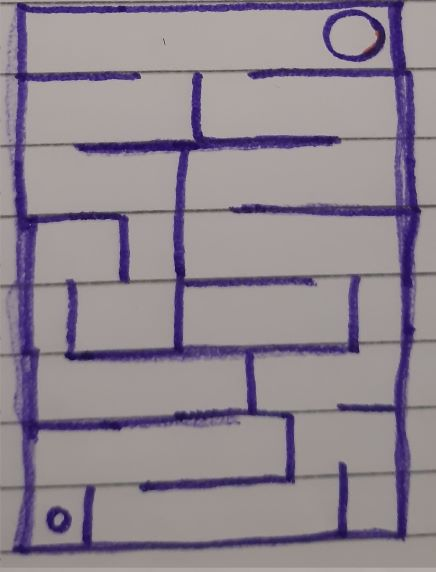
\includegraphics[scale=0.25]{medium.jpg}
    \label{fig:medium}
    \caption{Labirinto de entrada}
    }
\end{figure}

\subsection{Suavização do ruído}
 Para suavizar primeiramente tornou a imagem original em uma de tons de cinza e depois foi usado um filtro gaussiano com um kernel pequeno. Isso se deve por dois motivos, o primeiro para que as paredes não fossem muito suavizadas com o fundo da imagem, o que dificultaria o processo de binarização; em segundo para que os círculos e paredes não se fundissem, o que dificultaria remover os círculos sem remover as paredes próximas a eles.

 \subsection{Binarização}
 Como a imagem de entrada tem como presunção que o fundo é mais claro que as paredes, ao usar a binarização de Otsu, todos os casos funcionaram como esperado. Veja figura 2.
 \begin{figure}[h!]
   \centering
    {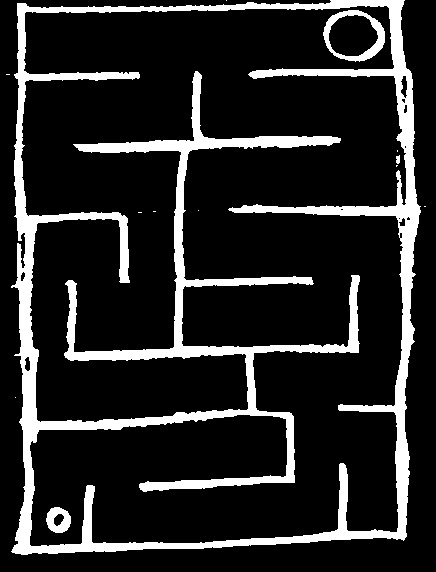
\includegraphics[scale=0.25]{edgeImagemedium.jpg}
    \label{fig:medium}
    \caption{Binarização da imagem entrada}
    }
\end{figure}
\subsection{Identificação dos pontos de início e chagada}
Para isso foi usado o Hough para detectar os círculos. Para acelerar a busca, limitou-se o tamanho máximo e mínimo do raio do círculo, pois os círculos não são muito grandes já que eles precisam ser menor que o largura do caminho do labirinto. Detectando os dois círculos se assume que o maior é o ponto de chegada e o menor o ponto de início.
 \begin{figure}[h!]
   \centering
    {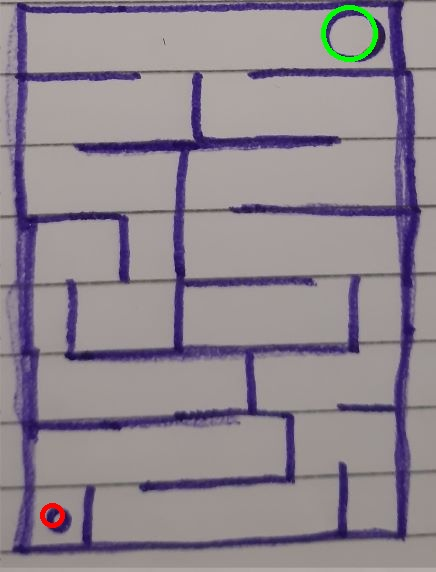
\includegraphics[scale=0.25]{edgeImageWithoutCirclesmedium.jpg}
    \label{fig:medium}
    \caption{Remoção dos pontos iniciais e finais da imagem entrada}
    }
\end{figure}
\subsection{Remoção dos círculos da imagem}
Para que os círculos não atrapalhassem a busca pelas paredes do labirinto, eles foram removidos. Para isso, removeu-se um círculo com o raio maior do que o círculo encontrado, porque os círculos nas imagens podem ser defeituosos, já que podem ser feitos a mão ou ter um formato de elipse. O raio do circulo removido é uma porcentagem do raio do circulo.
\subsection{Identificação das paredes}
Para identificar as paredes do labirinto, também foi usado Hough. Como as paredes são perpendiculares e paralelas entre si, foi usado um espaço de busca dividido em 90º graus. Com a equação gerada por Hough e com base na imagem, se detectou os pontos iniciais e finais de cada linha gerada por Hough, essas linhas representam as paredes.
\subsection{Unificação de paredes próximas}
O algoritmo de Hough nem sempre retorna uma linha representando uma parede, as vezes o retorno é um conjunto de linhas para representar-la, principalmente quando as paredes são largas e extensas, como as paredes externas, sendo assim, era preciso unifica-las.

Então para unifica-las, primeiramente se separou as linhas em dois grupos, as das paredes horizontais e as das verticais. Depois se pegava uma linha e analisava, no caso de uma linha horizontal, dentre as outras linhas horizontais as que tinham o \(y\) parecido com a linha original e que tinha o valor de \(x\) uma de suas extremidades dentro, ou muito perto, dos valores de \(x\) da linha original. Então se atualizava o valor das extremidades com a nova linha e seguia até passar por todas as linhas.

Se uma linha tivesse no mesmo \(y\) da original mas não no intervalo de \(x\) se adicionava num conjunto de que ainda seria possível "alcançar" ela caso outras linhas fossem adicionadas a essa linha estendendo seu comprimento. E sempre que as extremidades mudavam, esse conjunto de linhas possíveis era adicionado no conjunto de linhas. O mesmo se aplica para as linhas verticais, só mudando os eixos.

Veja figura 4.
 \begin{figure}[h!]
   \centering
    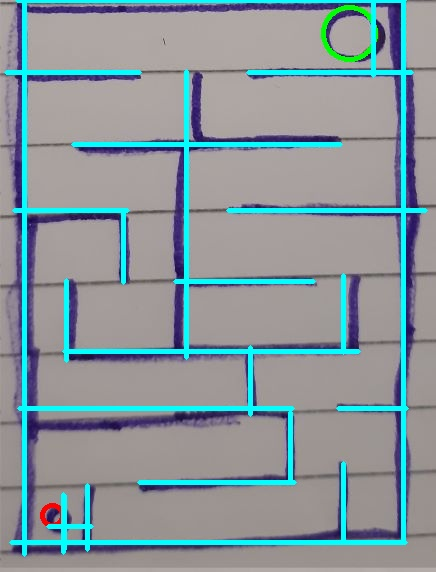
\includegraphics[scale=0.25]{lineImagemedium.jpg}
    \label{fig:medium}
    \caption{Paredes detectadas da imagem entrada}
\end{figure}
\subsection{Redução do labirinto para uma matriz}
Agora contendo as linhas representando as paredes, tentou-se deixar as linhas, que fossem na mesma orientação e tivessem o \(x\) ou \(y\) parecidos, com o mesmo valor, dessa forma essas paredes ficariam na mesma linha ou coluna da matriz quando acontecesse a redução, e não haver falsos buracos.

Depois que as linhas próximas foram padronizadas, se viu a menor distância entre linhas horizontais ou verticais, e isso se definiu o tamanho do bloco. Então a imagem foi discretizadas em blocos com o tamanho determinado anteriormente. Se um bloco tiver uma parede em mais de metade do tamanho dele, ele inteiro vira uma parede, se naquele bloco tiver o centro de um dos pontos de inicio ou chegada, ele vira o bloco de começo ou fim. Senão vira um bloco livre, onde o caminho da solução poderia passar.  Veja figura 5.
 \begin{figure}[h!]
   \centering
    \includegraphics[scale=0.25]{matrixMedium.png}
    \label{fig:medium}
    \caption{Matriz gerada da imagem entrada.}
\end{figure}


\subsection{Resolução do labirinto}
Com uma matriz representando o labirinto, foi usado o algoritmo A* para resolver o caminho do ponto de inicio ao ponto de chegada do labirinto.
\subsection{Desenhar a solução no labirinto}
Tendo o caminho gerado pelo passo anterior e sabendo que a solução só pode andar para 4 direções, bastou desenhar uma linha do ponto médio de cada bloco até o ponto médio do próximo bloco na solução.
\begin{figure}[h!]
   \centering
    {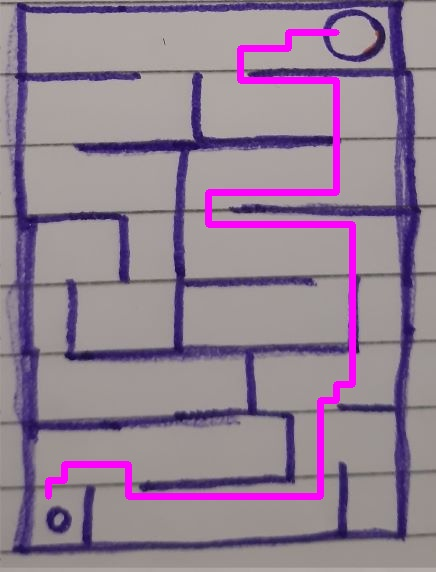
\includegraphics[scale=0.3]{solutionmedium.jpg}
    \label{fig:solutionmedium}
    \caption{Solução labirinto de entrada}
    }
\end{figure}

\section*{Resultados experimentais}
Segue em anexo as imagens de saída do solucionador de labirintos, nas quais em rosa está o caminho encontrado como solução (Figuras 7 a 9).
\begin{figure}[h!]
   \centering
    {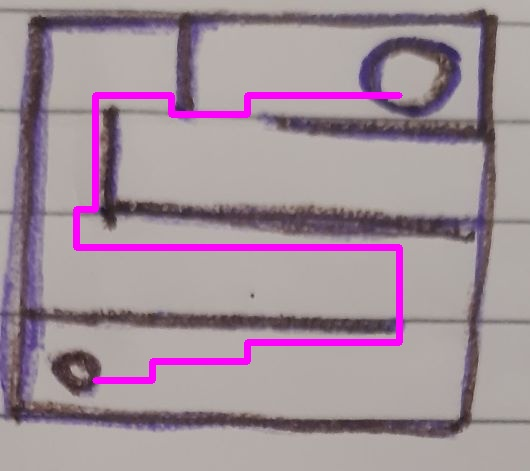
\includegraphics[scale=0.25]{solutioneasy.jpg}
    \label{fig:solutioneasy}
    \caption{}
    }
\end{figure}

\begin{figure}[h!]
   \centering
    {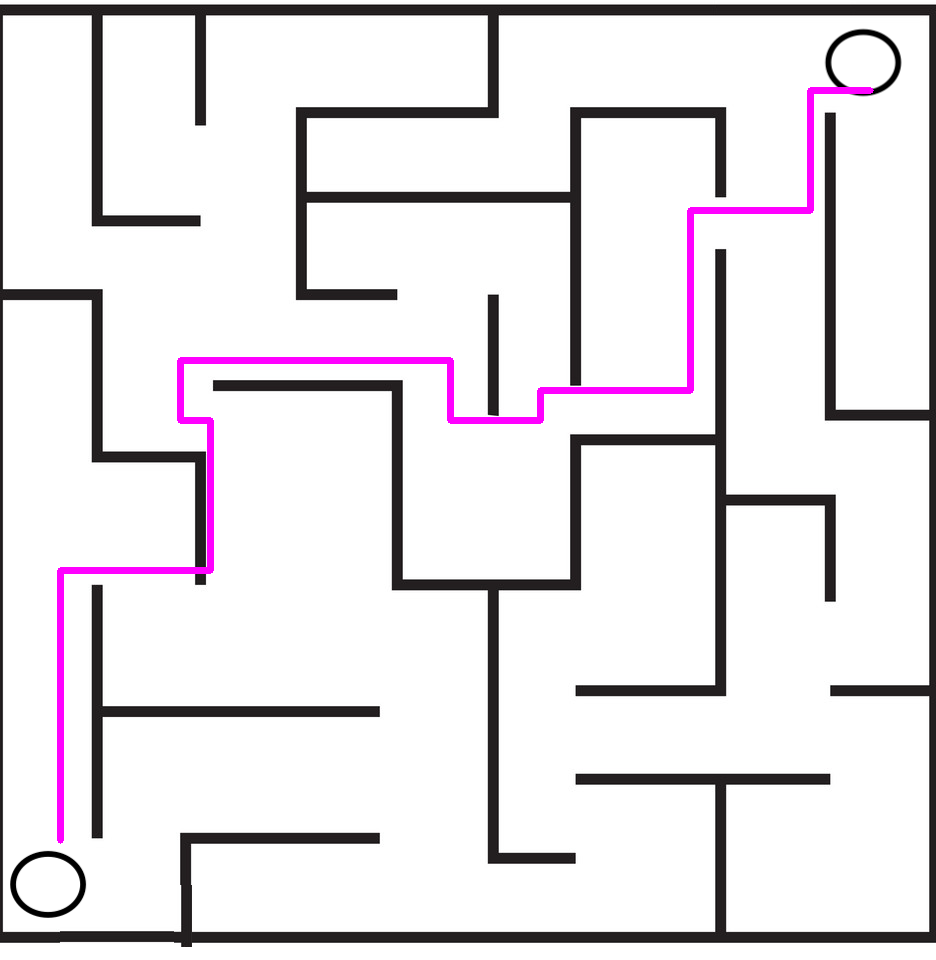
\includegraphics[scale=0.15]{solutionhard.png}
    \label{fig:solutionhard}
    \caption{}
    }
\end{figure}
\begin{figure}[h!]
   \centering
    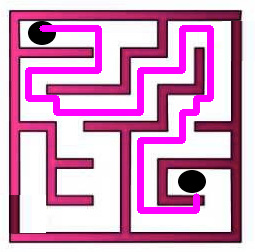
\includegraphics[scale=0.5]{solutionlab3.png}
    \label{fig:solutionlab3}
    \caption{}

\end{figure}

\section{Problemas encontrados}
    \subsection{Binarização}
    Não foi possível achar um valor fixo para a binarização ser efetiva em todos os exemplos. No exemplo Fig 10, as paredes não atingiam o threshold (conforme Fig 11), tornando impossível solucionar o labirinto. Mas se mudasse o valor manualmente para um menor, ele gerava normalmente uma solução para o labirinto (Fig 12).

    A solução final para esse problema, foi usar a binarização de Otsu, dessa forma não havendo mais problemas para essa figura em específico e em nenhuma outra.

        \begin{figure}[h!]
          \centering
            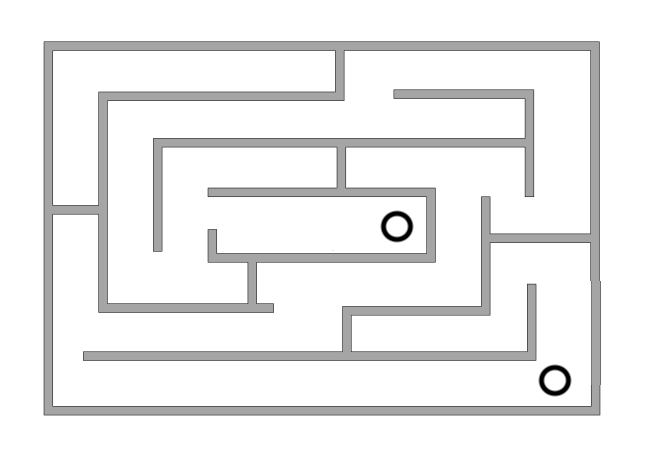
\includegraphics[scale=0.3]{lab2.png}
            \label{fig:lab2}
            \caption{Labirinto de teste com paredes cinza claro}
        \end{figure}
        \begin{figure}[h!]
            \centering
            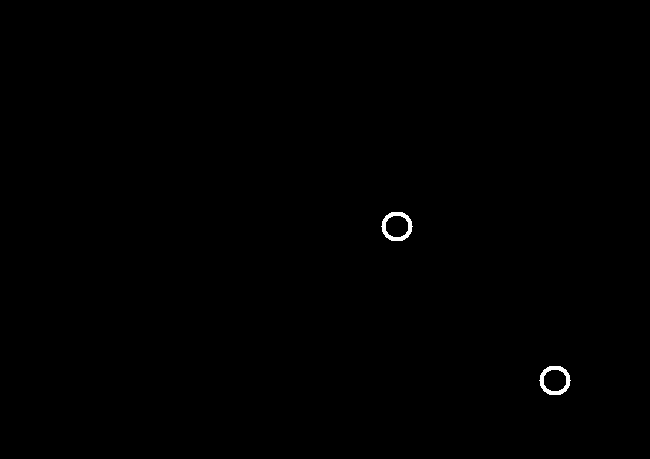
\includegraphics[scale=0.3]{edgeImagelab2.png}
            \label{fig:lab2Edge}
            \caption{Imagem da binarização da Fig 10}
        \end{figure}
        \begin{figure}[h!]
          \centering
            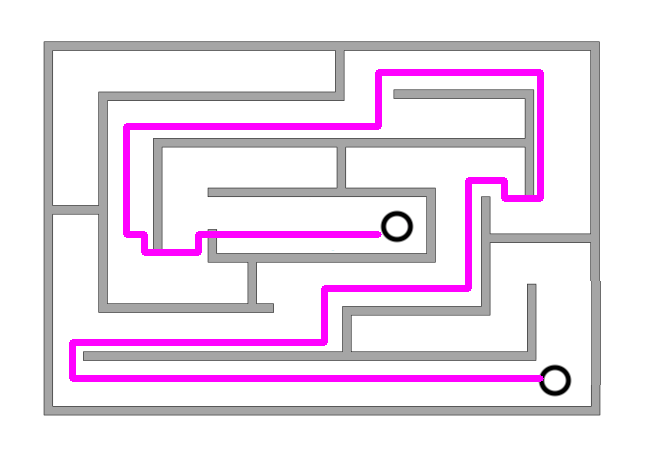
\includegraphics[scale=0.3]{solutionlab2.png}
            \caption{Solução da Fig 10}
        \end{figure}
    \subsection{Remoção dos pontos iniciais}
    Frequentemente a remoção dos pontos iniciais não ficava perfeita (Fig 14), podendo fazer com que o algoritmo detectasse paredes com o que sobrava dos círculos (Fig 13).

    Não foi implementada a solução desse problema, porém sabe-se que a utilização de componentes conexos resolveria, levando como premissa que nunca haverá um circulo encostado em uma parede.
     \begin{figure}[h!]
          \centering
            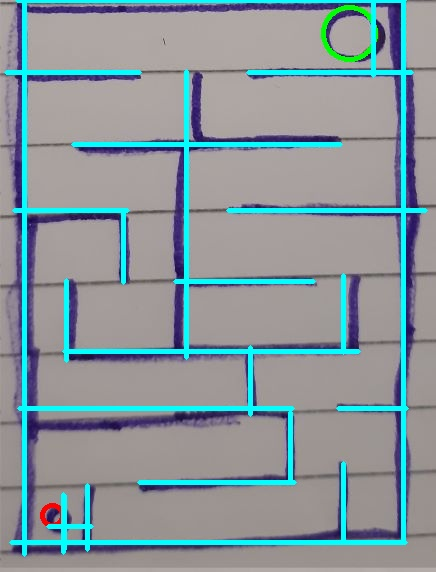
\includegraphics[scale=0.3]{lineImagemedium.jpg}
            \caption{Paredes falsas}
        \end{figure}
     \begin{figure}[h!]
          \centering
            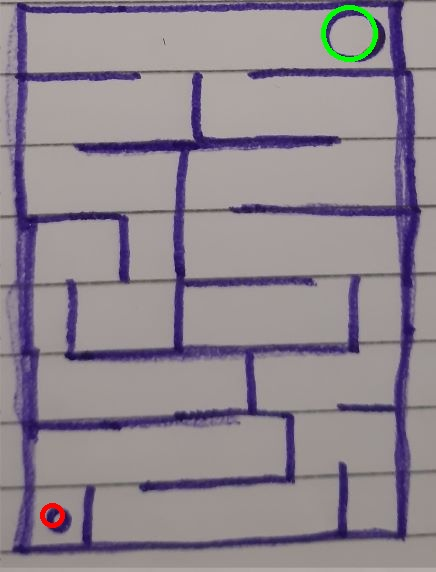
\includegraphics[scale=0.3]{edgeImageWithoutCirclesmedium.jpg}
            \caption{Imagem após remoção dos pontos iniciais}
        \end{figure}

    \subsection{Tamanho do bloco da matriz}
    Difícil encontrar o tamanho ideal dos blocos da matriz, ou seja, quanto um elemento da matriz representava em pixeis 2D. Porque se era de tamanho muito grande, poderia desconsiderar alguns espaços entre paredes por serem menores que bloco. Já quando o bloco era de tamanho pequeno, nos casos que a parede não chegava a encostar na outra, mas claramente não era um espaço possível para o caminho, a matriz considerava aquele bloco não sendo parede.

    A solução foi usar a menor espessura entre as paredes como tamanho do bloco.

\section*{Conclusão}

O algoritmo funciona bem para labirintos onde as paredes são escuras e o fundo é claro. A parte mais complicada foi tentar achar um valor único para binarização funcionar com todas imagens, o que foi resolvido com Otsu.

O solucionador de labirintos foi implementado com técnicas relativamente simples de visão computacional e seu resultado foi bem satisfatório. Mas, sabe-se que se fosse usado algumas outras técnicas um pouco mais elaboradas, como por exemplo, componentes conexos ao invés de apenas o circulo detectado por Hough no momento de remoção dos círculos de início e chagada, haveria melhores resultados.


\begin{thebibliography}{00}
\bibitem{b1} https://docs.opencv.org/3.4/d9/db0/tutorial_hough_lines.html

\bibitem{b2} https://docs.opencv.org/3.4/d4/d70/tutorial_hough_circle.html

\bibitem{b3} https://www.laurentluce.com/posts/solving-mazes-using-python-simple-recursivity-and-a-search/
\end{thebibliography}

\end{document}
